\chapter{Scelte progettuali}
\label{chap:ScelteProgettuali}
\section{Scelta modello di sviluppo}
La scelta del modello di progettazione è ricaduta in un modello agile.
Questa scelta è statq dettata principalmente dalla necessità di avere in breve tempo un prototipo
da testare con il richiedente.
La progettazione è stata suportata dalla creazione di Unit Test.
I test sono stati fondamentaliper poter validare il codice,
in particolare a fronte di aggiornamneti della struttura database.
Nel corso dell'implementazione, soprattuto della view, si è spesso seguito un pattern tipico del modello ovvero:
\begin{enumerate}
    \item Creazione del prototipo della funzione.
    \item Creazione della view di riferimento.
    \item Test e validazione da parte di un utente scelto.
    \item Rifattorizzazione codice se necessario.
\end{enumerate}
La rifattorizzazione del codice è stata affrontata con regolarità per seguire il principio\ac{DRY},
 favorendo aggiornamneti più agili a fronte di manuntezione di parti di codice.
\section{Suddivisione e contenuto dei rilasci}
La definizione delle tempististiche di rilascio è stata
supportata da un figura di Project Management messomi a disposizione.
Nel primo rilascio concordato sono compresi solo i requisiti che potessero almeno emulare gli attuali.
In questo rilascio, con consegna stimata gennaio 2027, sono presenti le seguenti funzionalità:
\begin{itemize}
    \item Gestione utenti e permessi.
    \item Anagrafica clienti.
    \item Creazione delle offerte.
    \item Versioning offerte.
    \item Creazione ordini.
    \item Import ed export dati, da e verso altri database.
    \item Creazione reportistica.
    \item Gestione multiligua interfaccia applicativa.
    \item Prototipo mobile.
    \item Modulo di configurazione prodotto.
\end{itemize}
Si è scelto di non includere la funzionalità offline
in quanto essa necessita di un database centrale stabile.
La funzione offline verrà implementata nel secondo rilascio quando il software sarà in produzione.
Nel secondo rilascio saranno presenti quindi;
\begin{itemize}
    \item Gestione revisione tecnica e differenze con contratto firmato.
    \item Inserimento calcoli automatici sulla base delle caratteristiche del venduto (ES: potenza elettrica totale assorbita).
    \item Gestione multi-valuta per ordini internazionali.
    \item Apertura disegni .pdf dal server del \ac{PLM}.
    \item Report avanzati.
    \item Implementazione database locale con logiche di sincronizzazione.
\end{itemize}
Le tempistiche di questo rilascio saranno stabite al
termine dei test del primo.
\section{Scelta Framework ORM}
All'interno della sezione \ref{chap:architettura} ho citato la scelta del framework \ac{MEF}.
Questo framework ha permesso di mappare le tabelle mediante la tecnica \ac{ORM}.
Questa tecnica consiste nel mappare ogn tabella del database in una classe 
e gestire tutti i legami mediante una classe context.
\Ac{ORM} ha permesso, mediante script powershell e connessione al database, 
di ricreare in modo dinamico tutte le entity a fronte di cambiamenti del database.
Tale approccio può essere definito database first, in quanto la progettazione avviene principalmente sul database, 
il software successivamente.
Le query mediante il framework \ac{MEF} sono state scritte tramite \ac{LINQ} che ha permesso di scriverle in linguaggio C#.
Queste funzioni sono inoltre utilizzabili anche con SQLite in ottica di offline.
All'interno degli aspetti negativi era presente la lentezza in grandi volumi dovuti alla traduzione del codice in query.
Si è valutato, in caso si presentino di ottimizare il database mediante indici in prima battuta
 e successivamente ottimizzando le songole query.

 \lstinputlisting[language=CSharp, caption={Esempio di query LINQ}]{listings/LINQ-example.cs}

\section{Scelta Framework grafico} % MAUI .NET
La scelta del framework relativo alla view utente era, come da requisiti, vincolata alla portabilità ed all'esecuzione offline.
La decisione era quindi ricaduta su due scelte principali ovvero:
\begin{itemize}
    \item Front end web based, con utilizzo di htlm, css, javascript e mediante api interrogare il database centrale.
    \item Utilizzo del Framework MAUI, nativamemente cross-platform ed integrato perfettamente con Backend.
\end{itemize}
La scelta dell'utilizzare una interfaccia web, utile per avere view che si addattano a dispositivi diversi,
 è stata bocciata principalmente per due motivi.
La difficoltà principale era l'utilizzo in locale. In assenza di connessione tutti i file ed il database locale devono essere presenti sul dispositivo stesso.
Questa caratterista rende difficoltoso gestire gli aggiornamenti.
Il secondo motivo è l'utilizzo di più linguaggi di programmazione che non massimizzano l'esperienza acquisita con altri moduli.
In ottica di ridurre la tempistica nell'avere un primo test con gli utenti essa era considerata un malus.
Il framework MAUI di .NET sopperisce ad entrambi i problemi.
Il programma è fisicamente installato sui dispositivi ed il loro aggiornamneto
 può essere gestito centralmente  all'intreno di uno store Microsoft.
 Essendo esso in base .NET e, mediante il framework "Comunity Toolkit Maui", le interfacce sono scritti in base C#.
\section{Scelta del pattern di progettazione} % MVVM
Insieme all'utilizzo di MAUI è suggerito da Microsoft il pattern \ac{MVVM}.
Il modello MVVM consente di separare in modo pulito la logica di business e presentazione 
di un'applicazione dalla relativa interfaccia utente.
La gestione di una separazione netta tra la logica dell'applicazione e 
l'interfaccia utente consente di risolvere numerosi problemi di sviluppo e semplifica il test, 
la gestione e l'evoluzione di un'applicazione. Può anche migliorare significativamente le opportunità 
di riutilizzo del codice e consente agli sviluppatori e ai progettisti dell'interfaccia utente di collaborare 
più facilmente durante lo sviluppo delle rispettive parti di un'app.\cite{MVVM}
Il modello \ac{MVVM} è composto da tre elementi fonamentali che interagiscono come segue:
\begin{figure}[h]
    \centering
    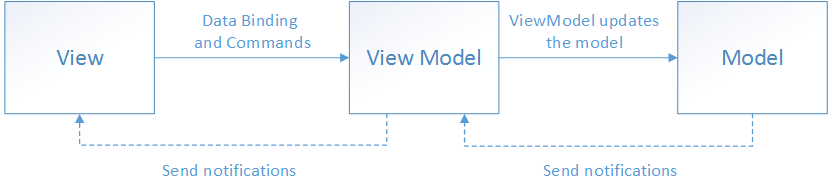
\includegraphics[width=1\linewidth]{figures/mvvm-pattern.png}
    \caption{Diagramma funzionamento MVVM}
    \label{fig:Diagramma funzionamento MVVM.}
\end{figure}
Questa modello, separando la logica della view da qeulla di bussiness,
ha permesso di protitipare le interfacce nei primi rilasci e in futuro riprogettarle
 migliorando l'accessibilità e \ac{UX}.